%%% Local Variables:
%%% mode: latex; mode: flyspell
%%% TeX-master: "."
%%% End:

\section { Fits }

To fit the end point value, convolved spectrums were generated for end point energies
between 80 MeV and 100 MeV using both detector response functions. The spectrums were scaled to minimize the $\chi^2$
or the negative log likelihood ($\mathcal{L}$), where the latter is able to take into account empty
bins in the data while the former cannot. For the $\mathcal{L}$, the convolved spectrum value was taken as the mean of
a Poisson distribution. The scale factors to minimize the $\chi^2$ and $\mathcal{L}$ fits were derived by:

$$f_{Poisson}(N;x_i) = \frac{x_i^N e^{-x_i}}{N!}$$
$$\chi^2 = \sum^N_{i=1} (\frac{A*x_i - y_i}{\sigma_i})^2; \mathcal{L} = -\sum^N_{i=1}log(f_{Poisson}(y_i;A*x_i))$$
$$\frac{\partial \mathcal{L}}{\partial A} = 0 \rightarrow A_{\mathcal{L}} = \frac{\sum^N_{i=1} y_i}{\sum^N_{i=1} x_i} $$
$$\frac{\partial \chi^2}{\partial A} = 0 \rightarrow A_{\chi^2} = \frac{\sum^N_{i=1} \frac{x_i*y_i}{\sigma_i^2}}{\sum^N_{i=1} \frac{x_i^2}{\sigma_i^2}} $$

\noindent
where $x_i$ is the predicted value corresponding to data $y_i$ for a given end point value.

The distribution of $\chi^2$ and $\mathcal{L}$ values as a function of the end point energy were each fit to a parabola near 
the minimum using ROOT to find the best fit end point value. The estimated uncertainty on the end point energy is then
defined by $\Delta \chi^2 = 1$ and $\Delta \mathcal{L} = \frac{1}{2}$. An example fit using the 1992 detector response function
and the 1992 aluminum data is shown in figure \ref{fig:1992AlFits}. The fit end point values for all 
datasets and both detector response functions are shown in figures \ref{fig:ChiSq} and \ref{fig:NLL}, and the $\chi^2$/DoF
distribution is shown in figure \ref{fig:ChiSqOfFits}. The $\chi^2$/DoF peaks around 1 for the 1998 detector response 
function and does not have the expected shape for the 1992 detector response function. Figure \ref{fig:compareFits}
shows the difference between these fits. Figure \ref{fig:ToyFitErrs} shows the errors in fitting toy data generated with
an end point value of 90 MeV. The toy fits shows that the expected difference between the $\chi^2$ and $\mathcal{L}$ fits is around 0.5 MeV.
The difference between the two fits for the data is around 1 MeV for the fits using the 1998 detector response function,
which is larger than expected but not too far off. The difference between the fits when using the 1992 detector response function
is around 3 MeV, consistent with the 1992 detector response not describing the data well.
The toy data fits suggests that the $\mathcal{L}$ fit end point values are closer to the true value due to a bias of around 0.5 MeV 
in the $\chi^2$ fits.

%%  where the $\mathcal{L}$ fit end point values are consistently higher which is consistent
%% with $\mathcal{L}$ being more sensitive to bins with low entries.

%% The published data was fit using both of the published response functions.
%% The method to fit the data was to minimize the $\chi^2$ value for many values
%% of kMax, and then fit a parabola to the $\chi^2$ distribution, 
%% $\chi^2_{Min} + \frac{(k-kMax)^2}{\sigma^2}$. The uncertainty on the fit kMax
%% is then the inverse square root of the coefficient. This was also done using
%% a negative log likelihood ($\mathcal{L}$) minimization strategy, where the variance is half of
%% the inverse of the leading coefficient. 
%% The latter is able to take into account empty
%% bins in the data while the former cannot. The end point values for each target Z 
%% are shown in figure \ref{fig:ChiSq} and \ref{fig:NLL} using $\chi^2$ and $\mathcal{L}$ minimization
%% respectively, and the $\chi^2$/DoF is shown in figure \ref{fig:ChiSqOfFits}. The $\mathcal{L}$
%% fitting method includes empty bins, which are ignored by the $\chi^2$ fitting method,
%% and has a greater cost for deviating from bins with small entry numbers. This results
%% in the $\mathcal{L}$ fit end point values being consistently higher, as is shown in figure \ref{fig:compareFits}.

\begin{figure}[h]
  \centering
  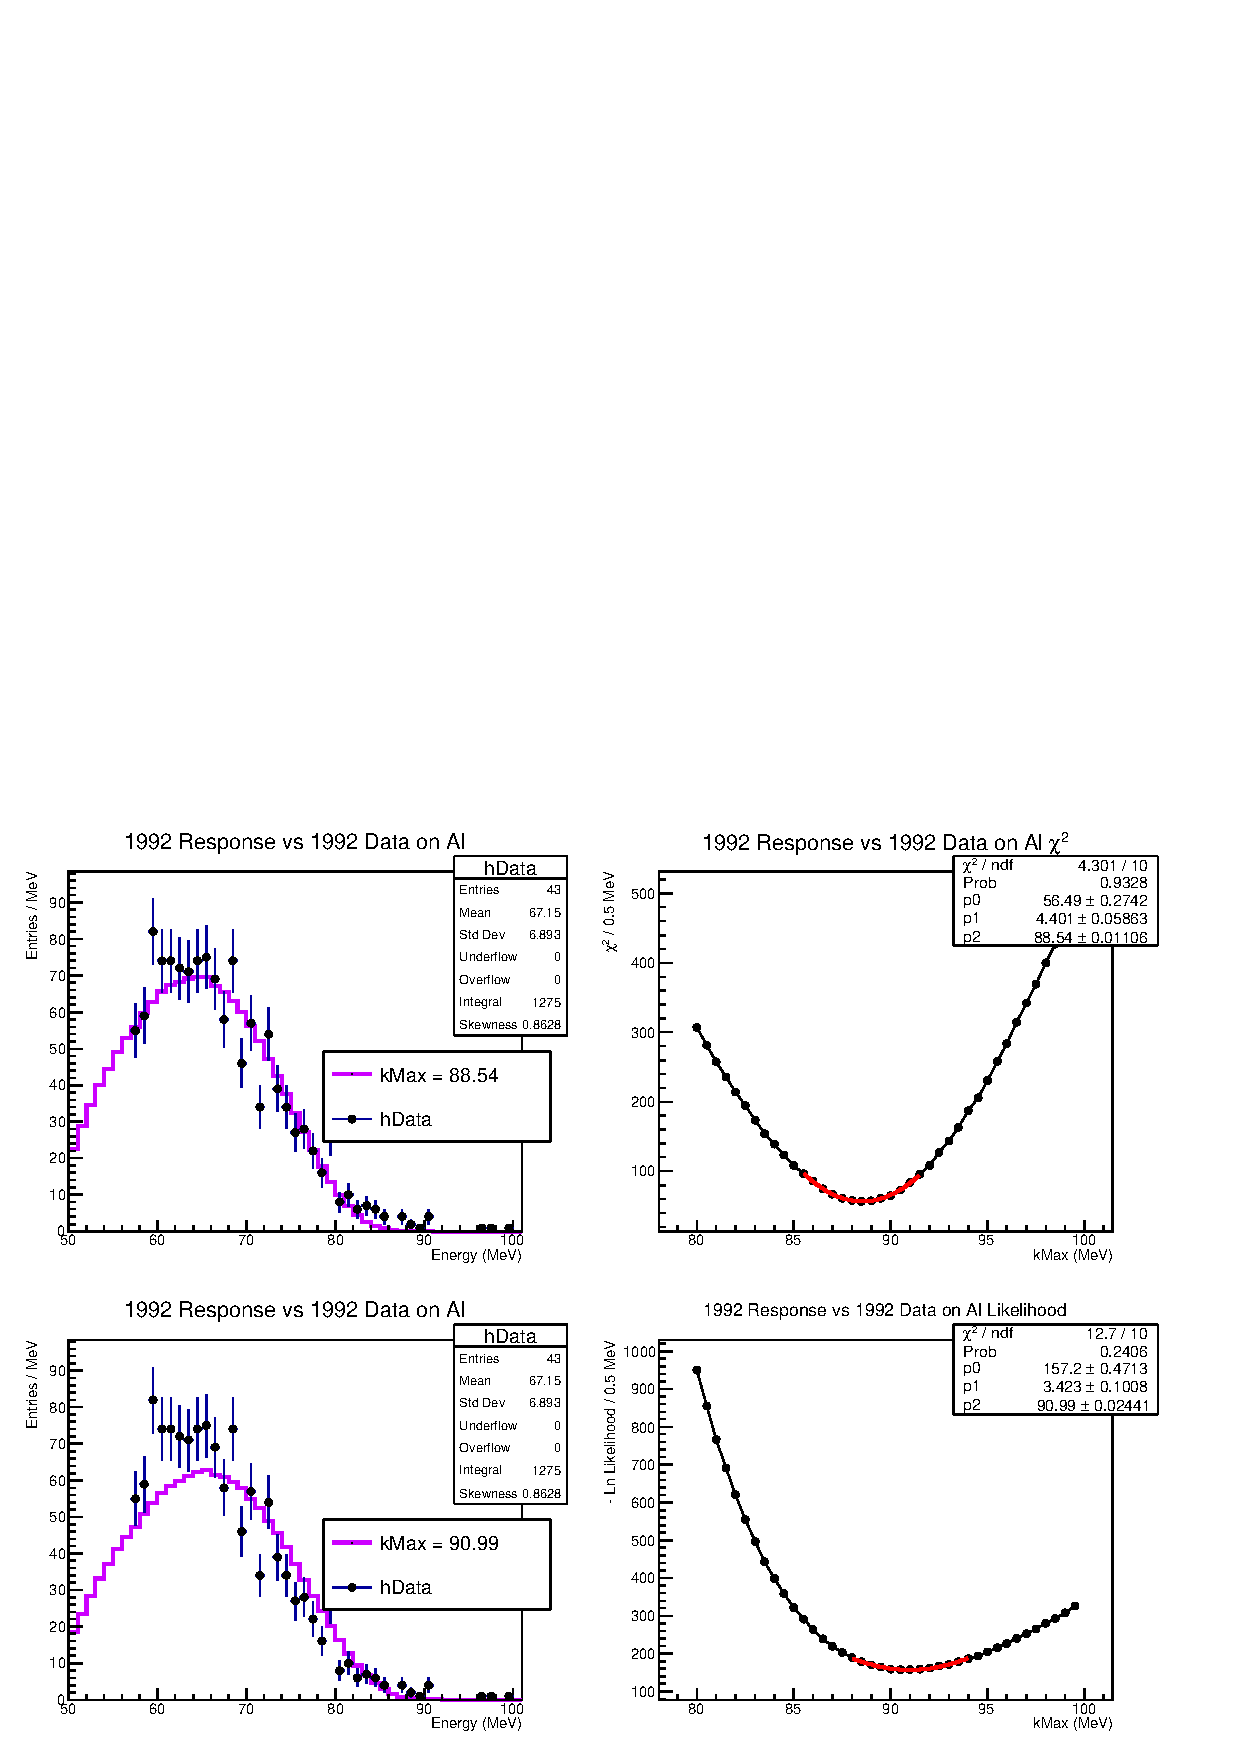
\includegraphics[width=0.8\linewidth]{figures/png/1992_resp_1992_Al_data_allPlots_singleK.png}
  \caption{The left figures show the best fit convolved closure approximation spectrum. The right figures
  show the parabolic fit to find the best fit endpoint value. The top figures use $\chi ^2$ 
  minimization while the bottom figures use $\mathcal{L}$ minimization.}
  \label{fig:1992AlFits}
\end{figure}


\begin{figure}[h]
  \centering
  \subfloat[ $\chi^2$ Minimization Fit \label{fig:ChiSq}]{%
  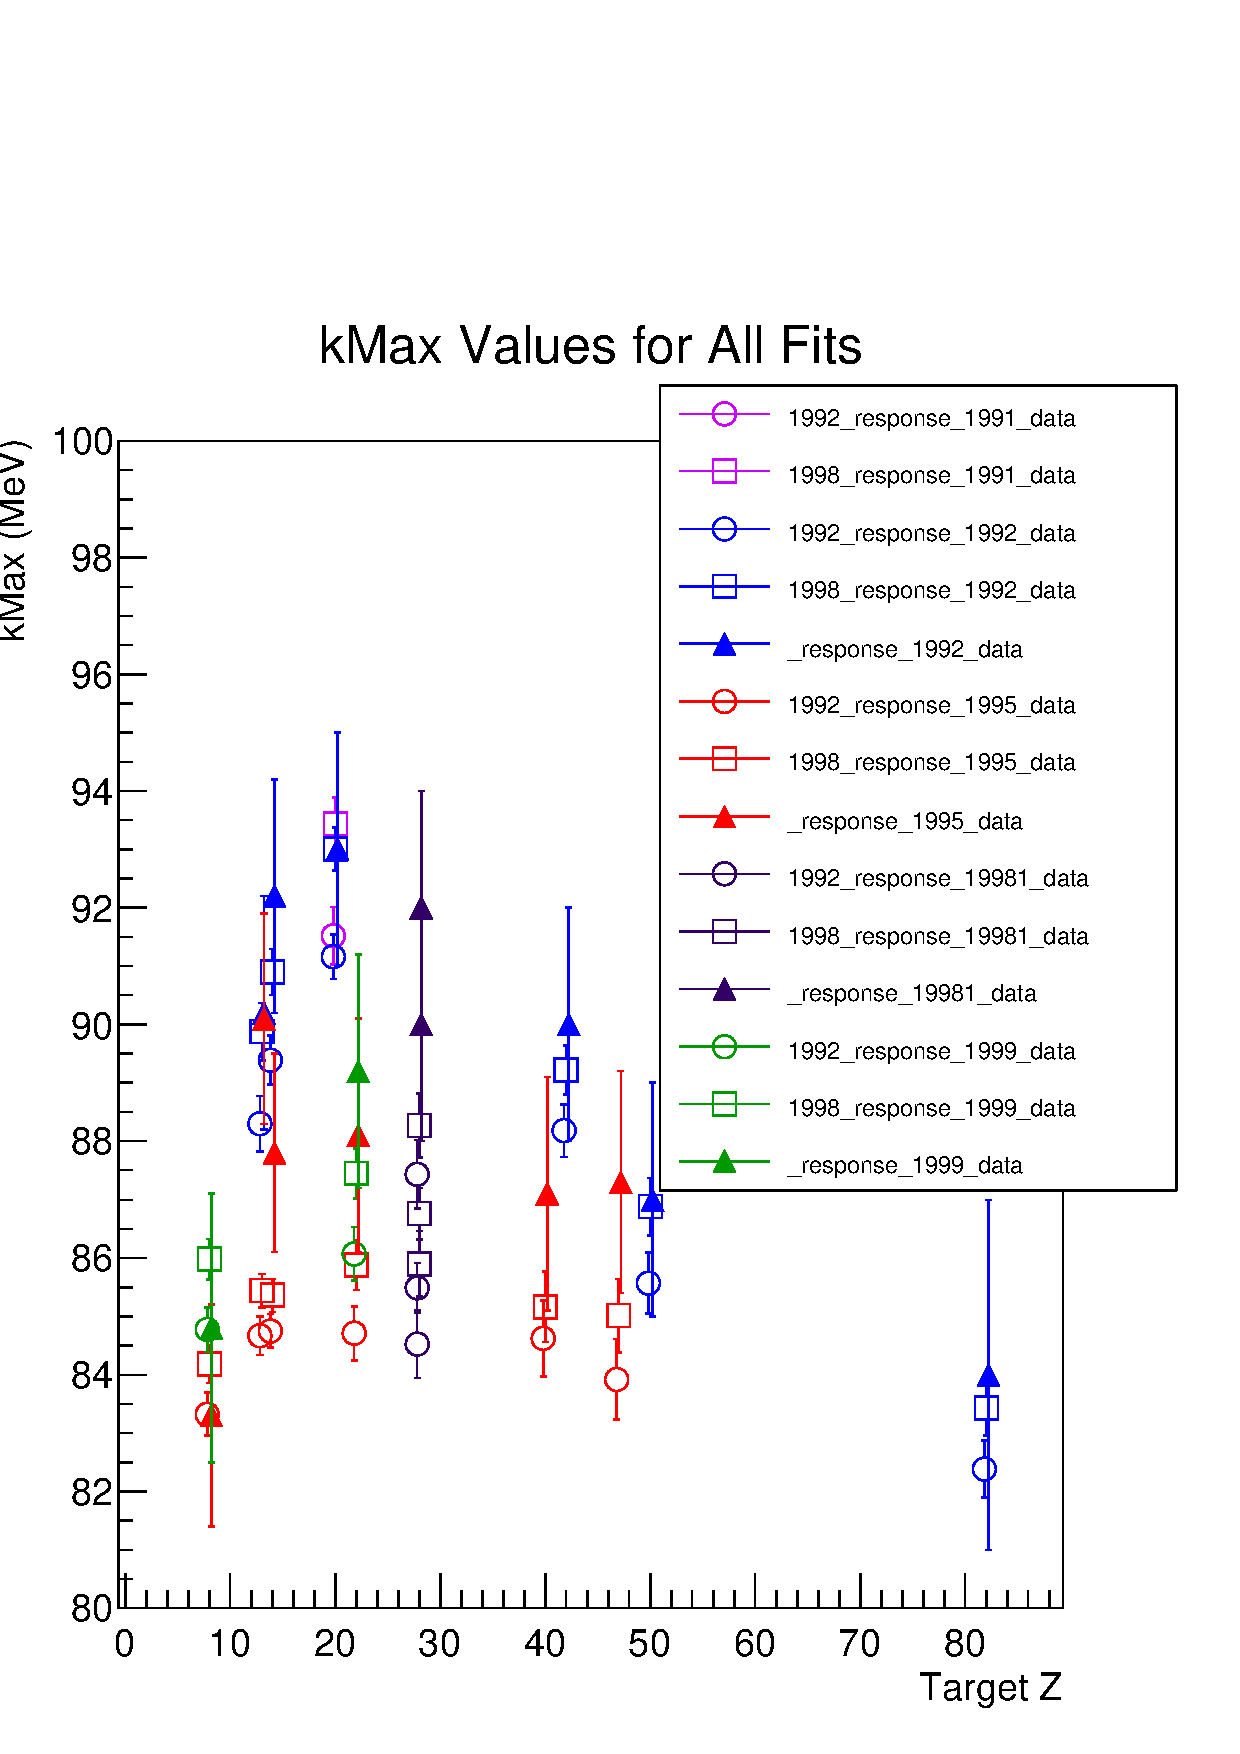
\includegraphics[width=0.48\linewidth]{figures/png/all_kMaxesChiSq_vs_target_z.png}
  }
  \hfill
  \subfloat[$\mathcal{L}$ Minimization Fit  \label{fig:NLL}]{%
  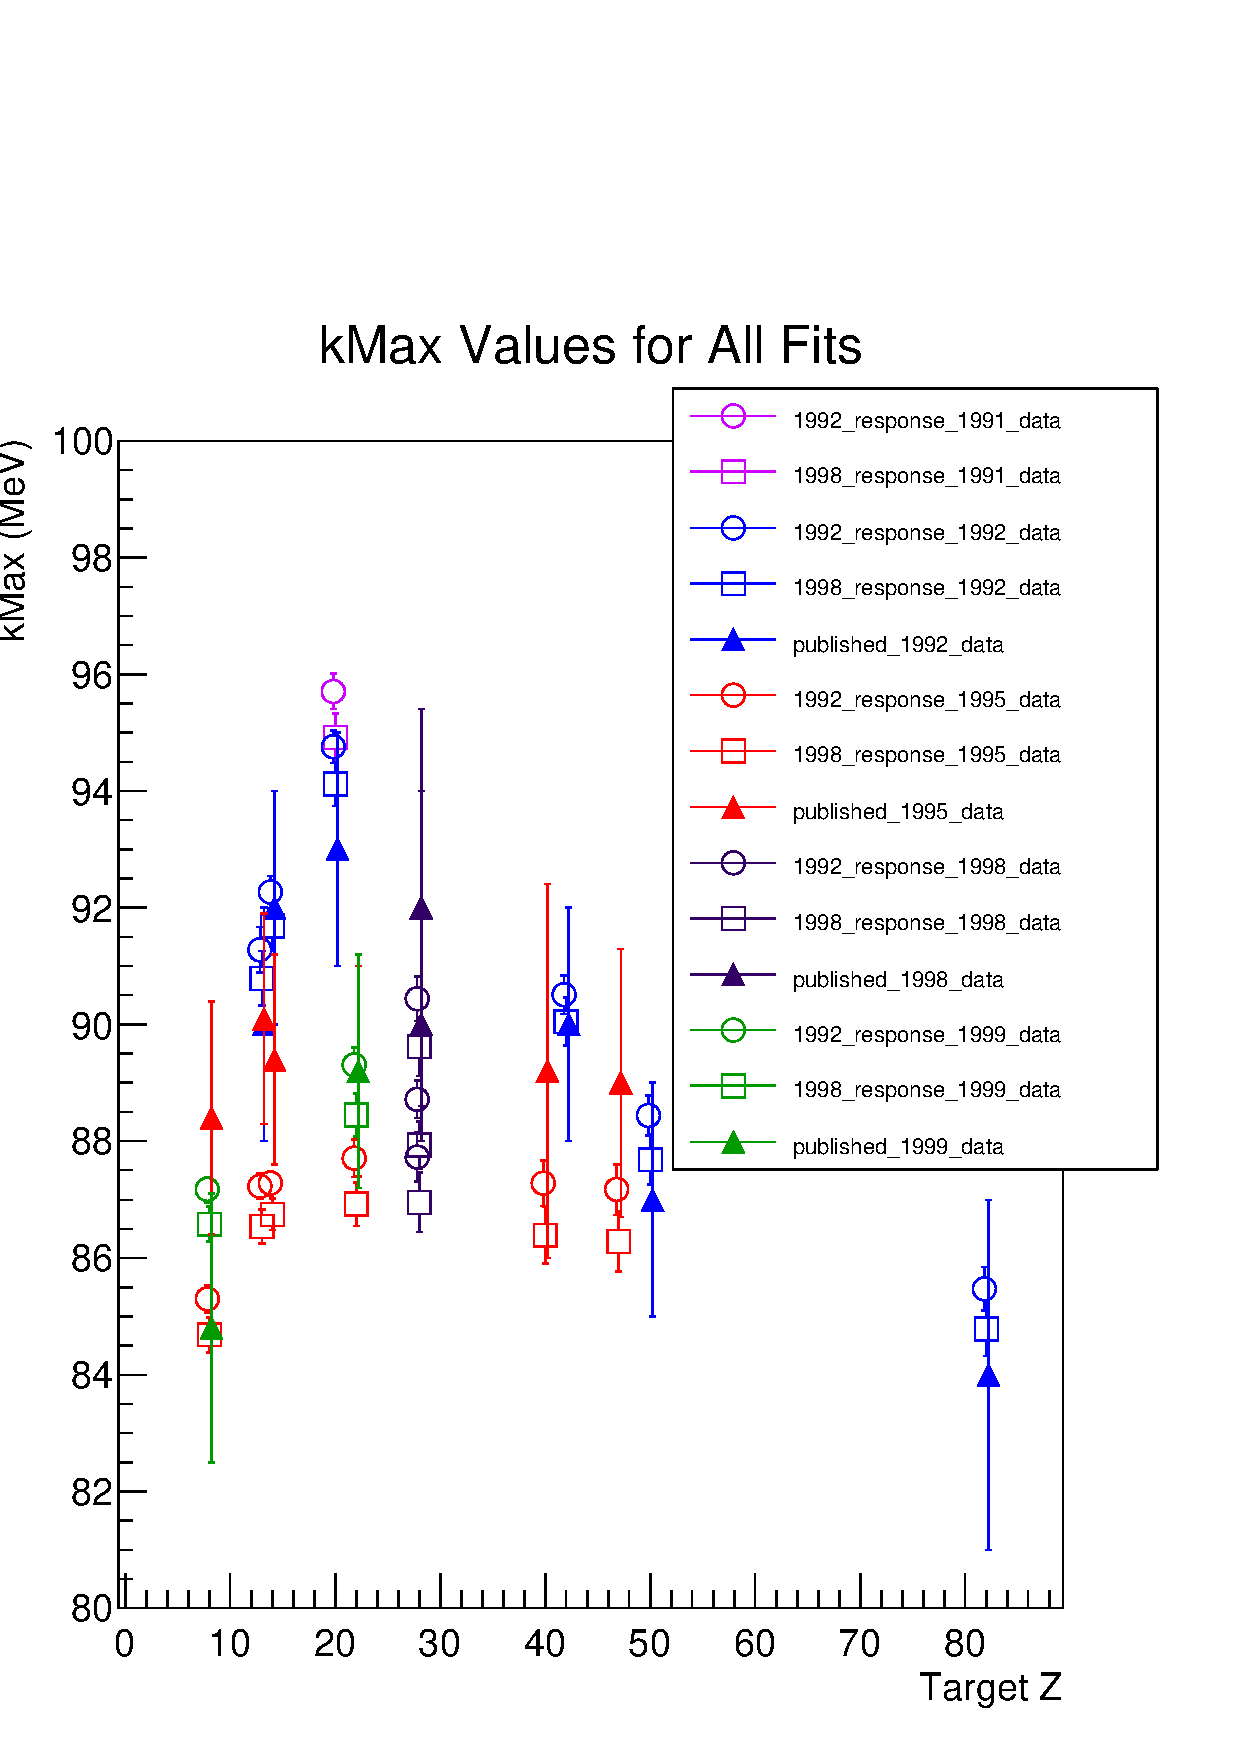
\includegraphics[width=0.48\linewidth]{figures/png/all_kMaxesNLL_vs_target_z.png}
  }
  \caption{Fit results vs target Z using (a) $\chi^2$ minimization and (b) $\mathcal{L}$ minimization.
    The 1992 detector response function data points (circles) are offset by -0.2 in z and the published data points (triangles)
    are offset by +0.2 in z.
  }
\end{figure}

\begin{figure}[h]
  \centering
  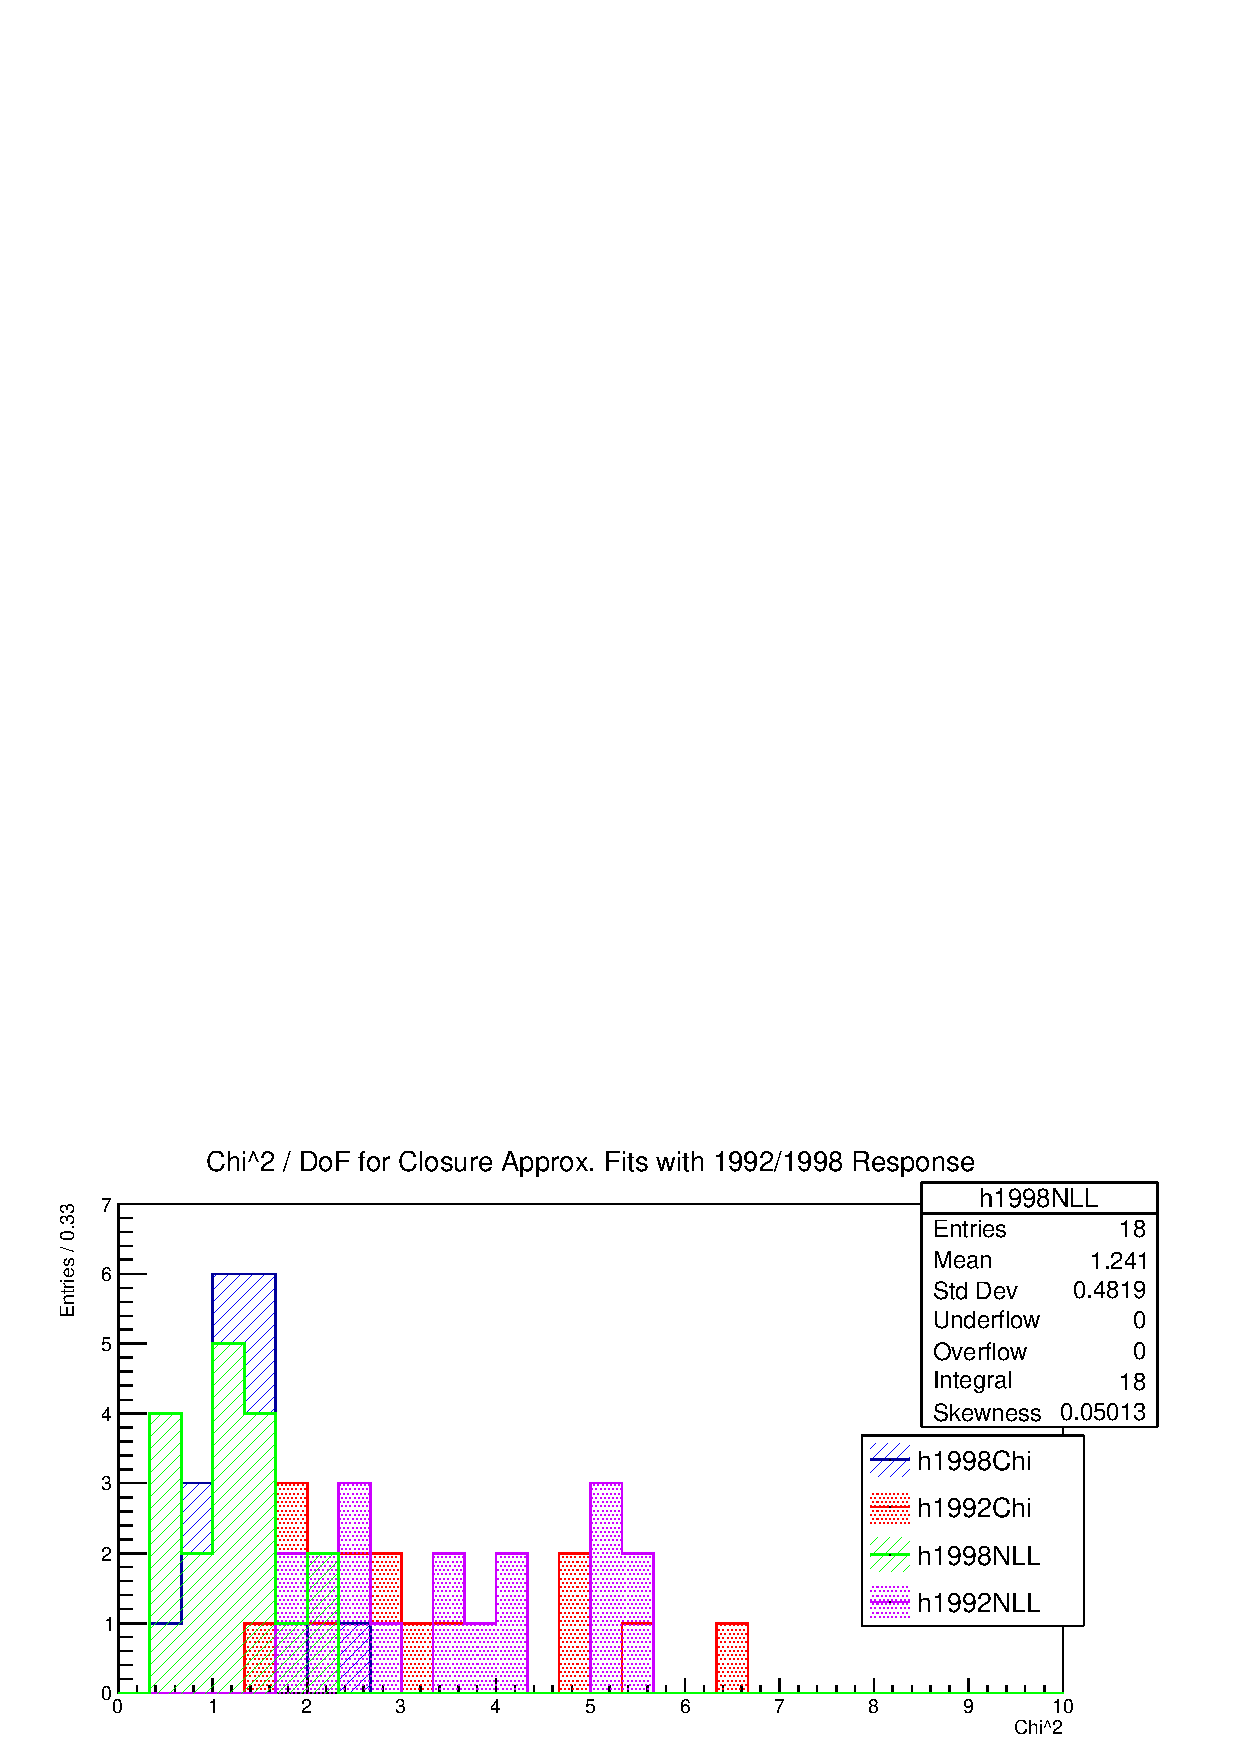
\includegraphics[width=0.8\linewidth]{figures/png/chiSq_of_fits.png}
  \caption{Fit $\chi^2$ values for both detector response functions and both fitting methods. }
  \label{fig:ChiSqOfFits}
\end{figure}

%% \begin{figure}[h]
%%   \centering
%%   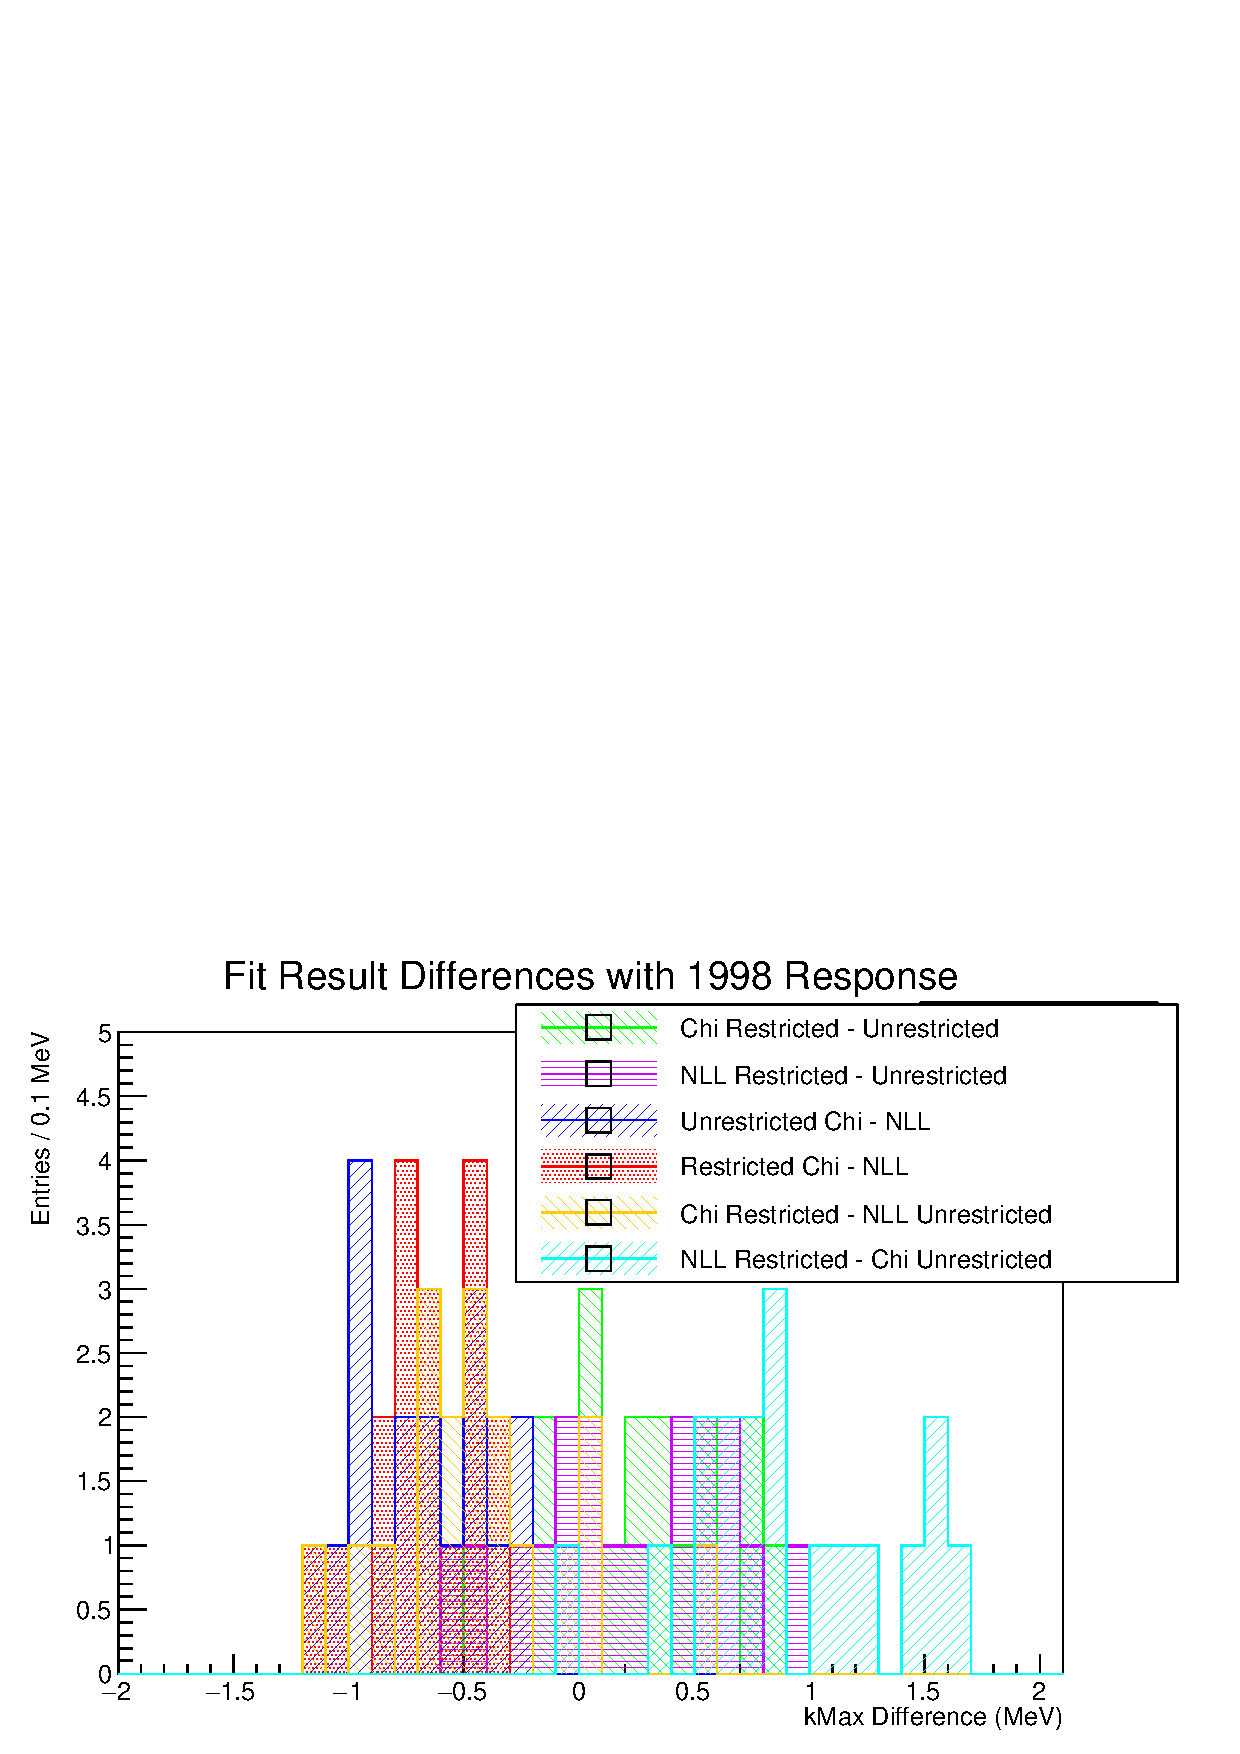
\includegraphics[width=\linewidth]{figures/png/compare_fit_results.png}
%%   \caption{Plot of the difference between the end point values found using $\chi^2$ and
%%     $\mathcal{L}$ minimization with and without a restricted range using the 1998 detector response function.}
%%   \label{fig:compareFits}
%% \end{figure}

\begin{figure}[h]
  \centering
  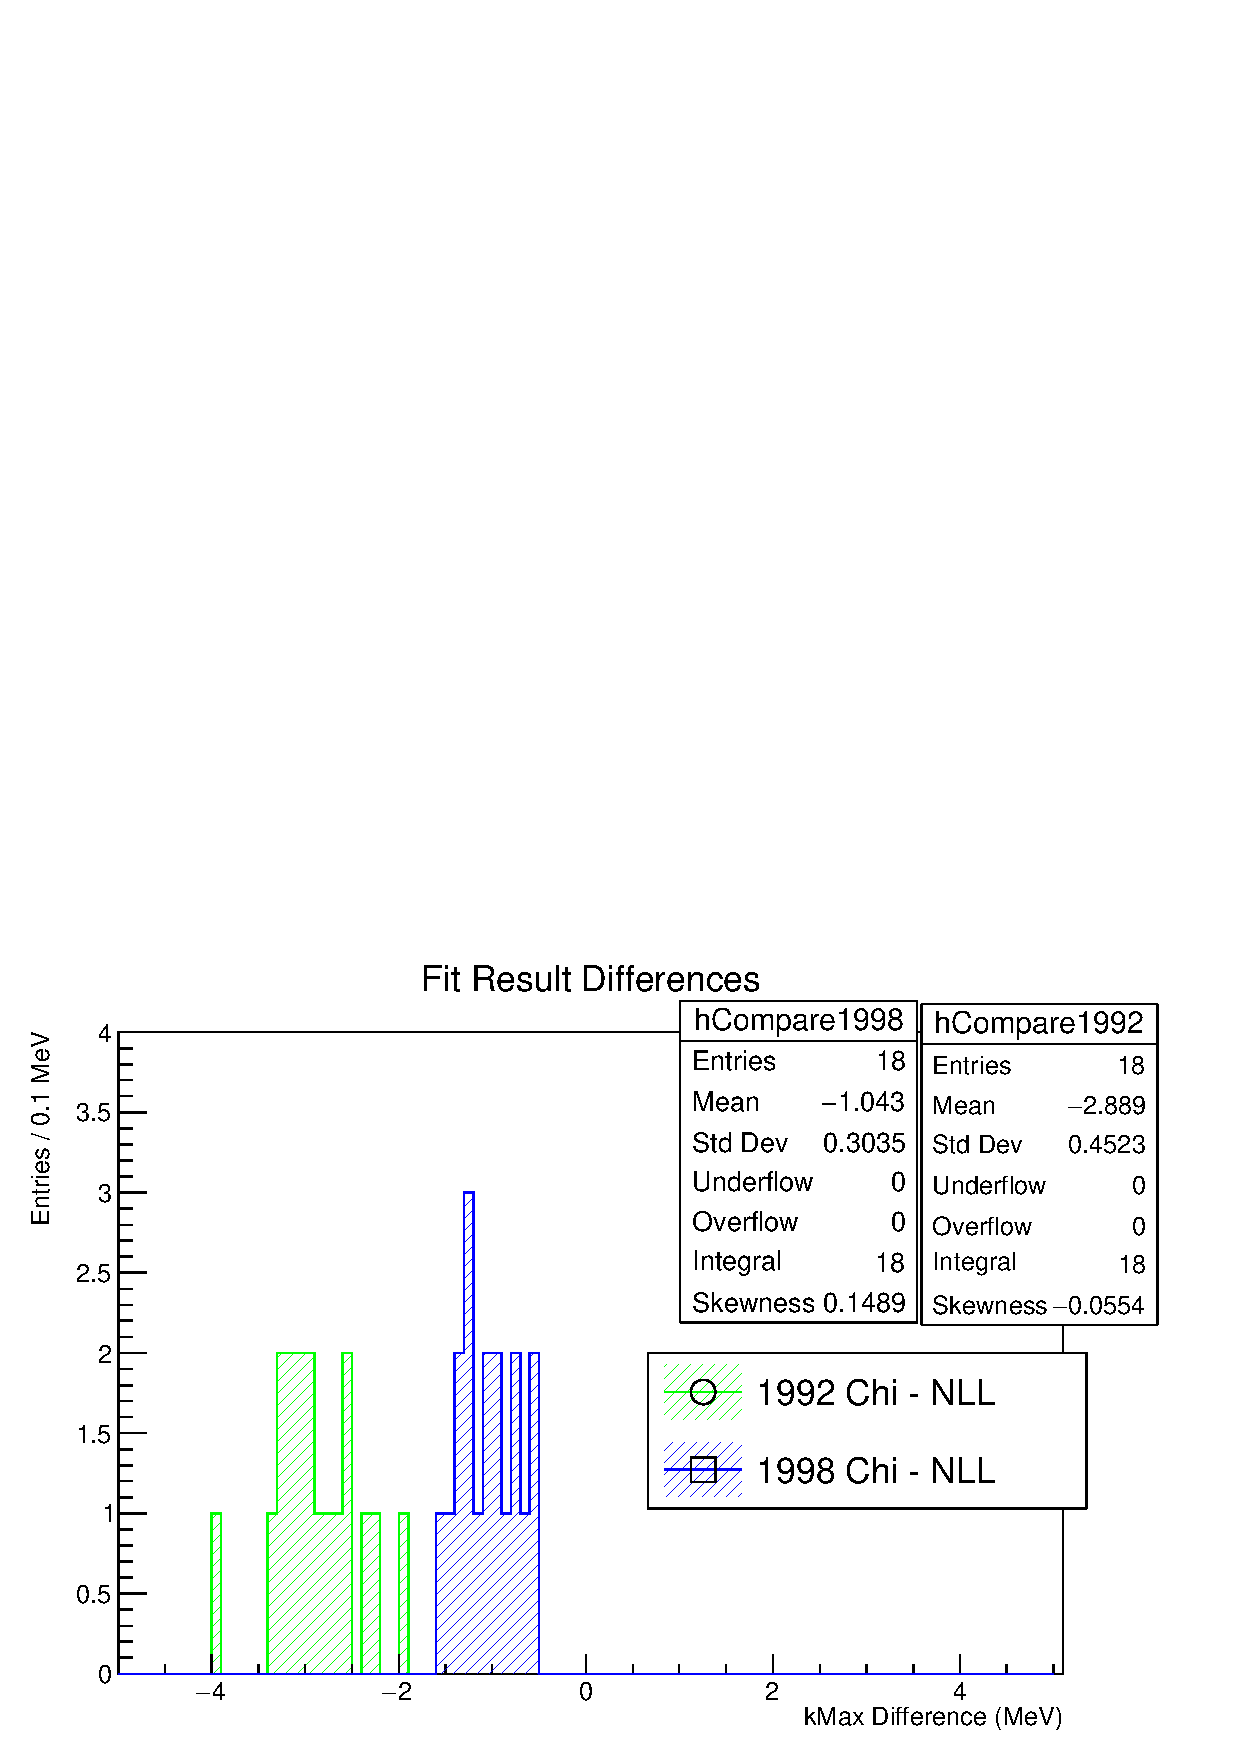
\includegraphics[width=\linewidth]{figures/png/compare_fit_results_92_v_98_unrestrictedOnly.png}
  \caption{Plot of the difference between the end point values found using $\chi^2$ and
    $\mathcal{L}$ minimization using the 1992 and 1998 detector response functions.}
  \label{fig:compareFits}
\end{figure}


\begin{figure}[h]
  \centering
  \subfloat[ 1992 detector response \label{fig:1992ToyErrs}]{%
  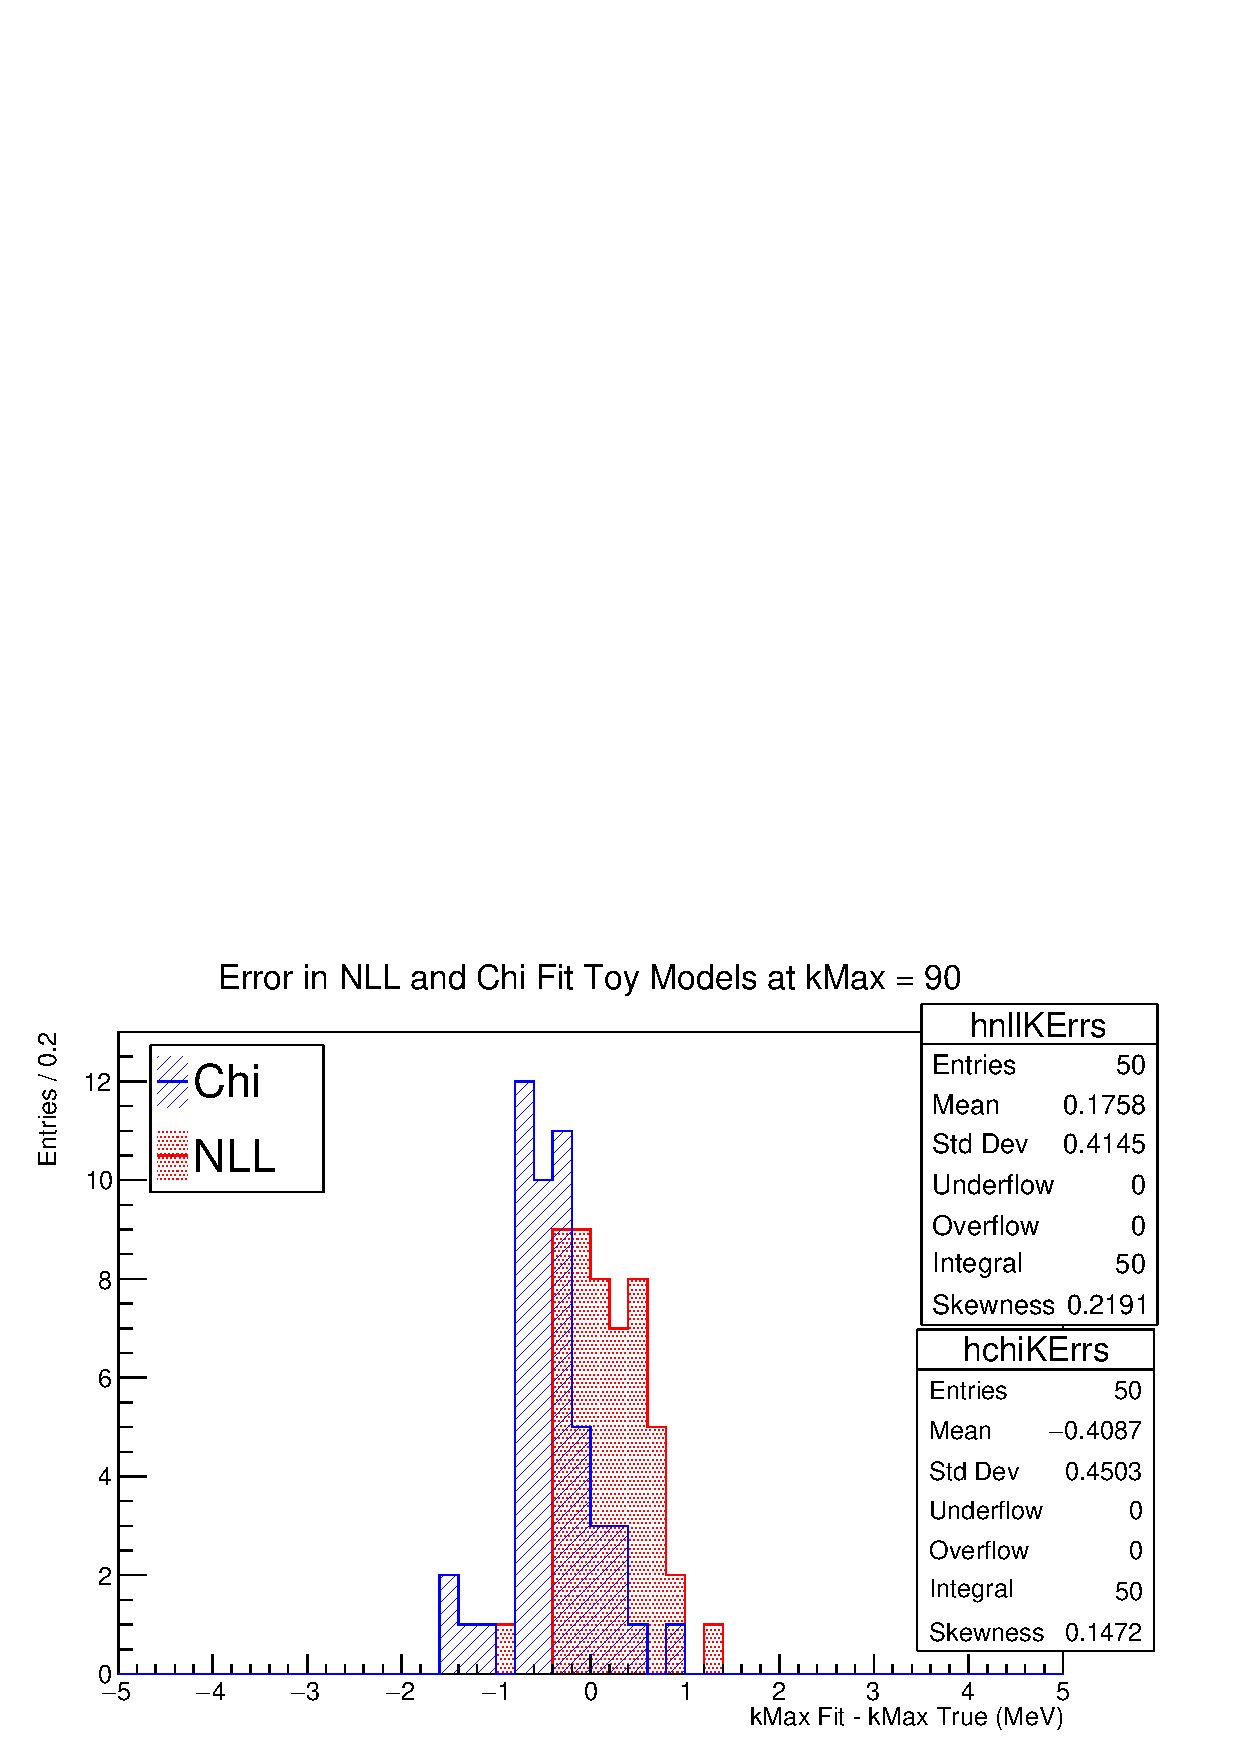
\includegraphics[width=0.48\linewidth]{figures/png/toy_kMax_errors_1992_response.png}
  }
  \hfill
  \subfloat[ 1998 detector response  \label{fig:1998ToyErrs}]{%
  \includegraphics[width=0.48\linewidth]{figures/png/toy_kMax_errors_1998_response.png}
  }
  \caption{Fit results errors for 50 toy data sets using the (a) 1992 or (b) 1998 detector response function.
    The toy data sets are generated from a convolution with an end point value of 90 MeV and generated
    with 1275 data points.
  }
  \label{fig:ToyFitErrs}
\end{figure}


%% \begin{figure}[h]
%%   \centering
%%   \subfloat[ 1992 detector response \label{fig:1992ToyZs}]{%
%%   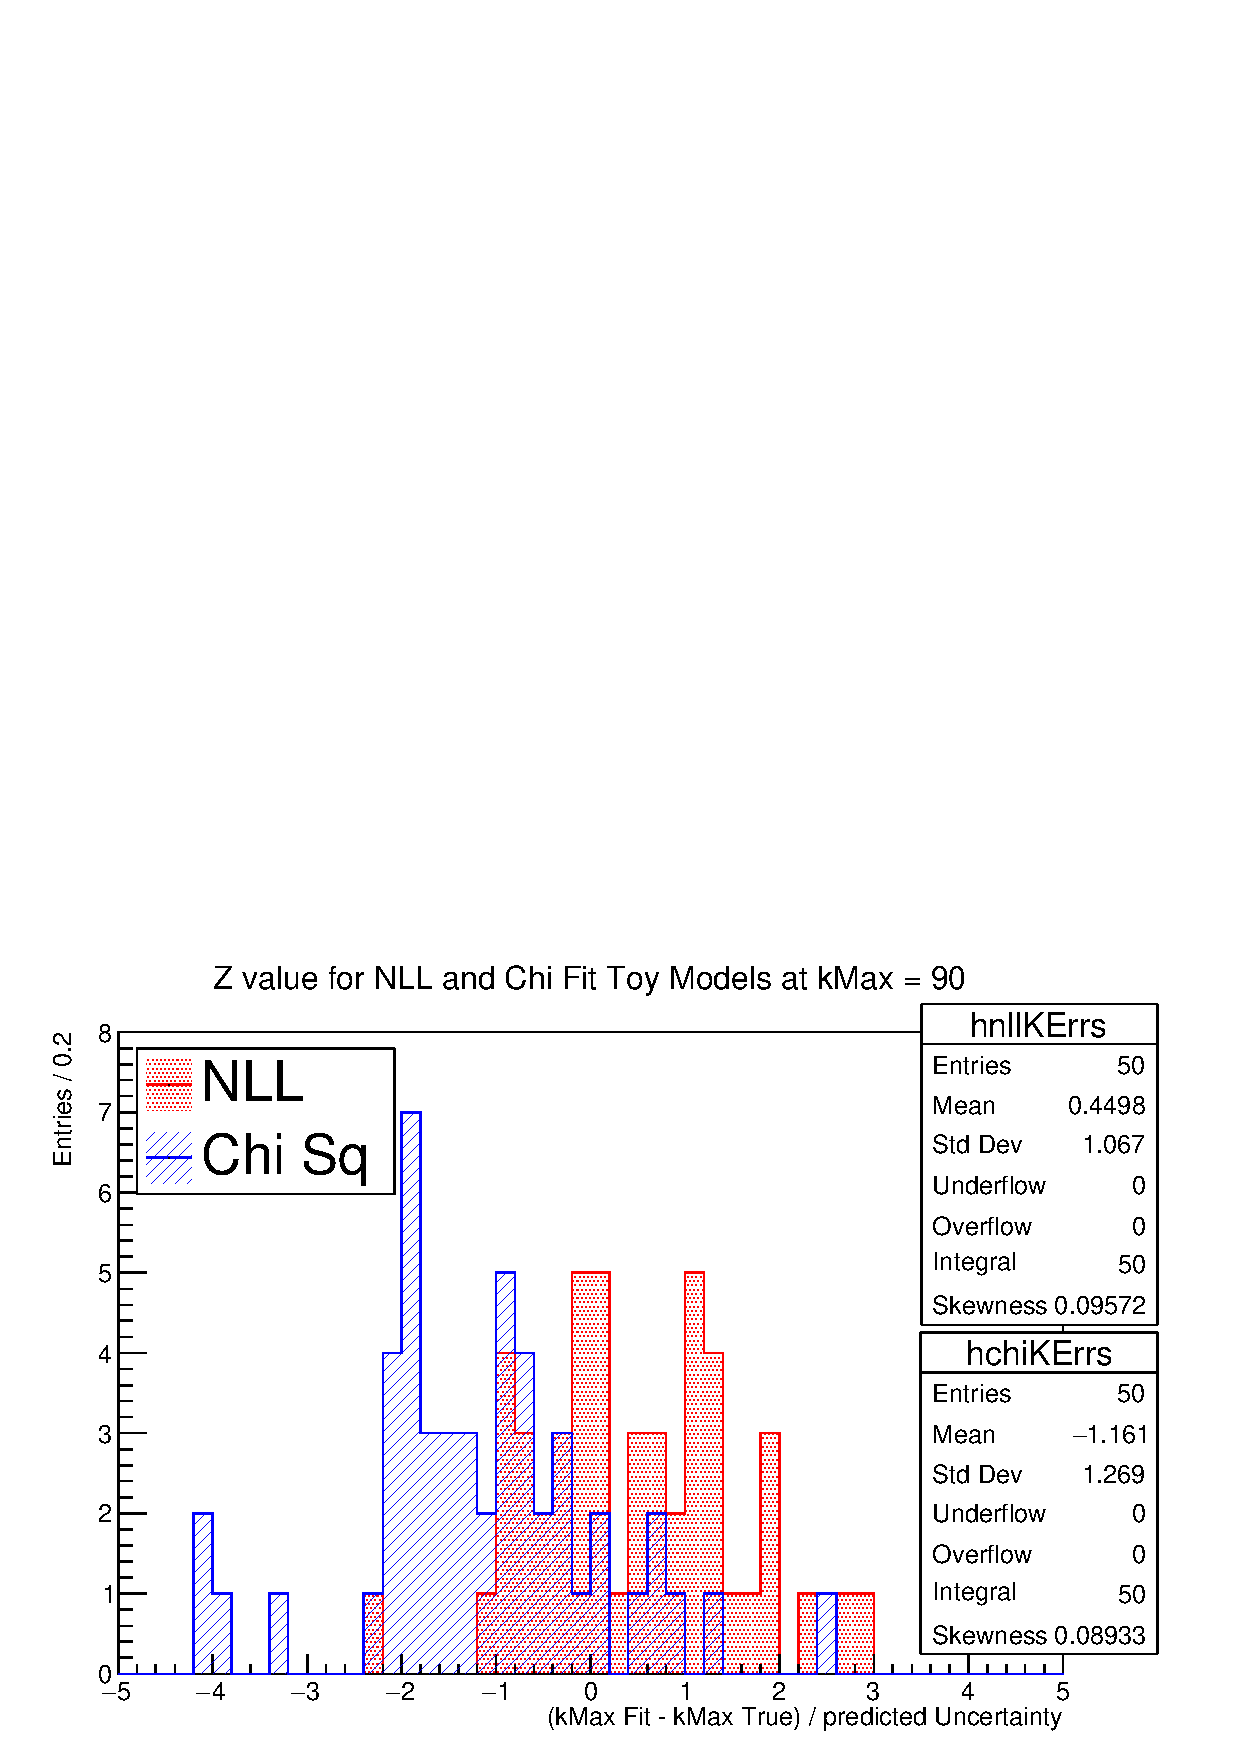
\includegraphics[width=0.48\linewidth]{figures/png/toy_kMax_z_values_1992_response.png}
%%   }
%%   \hfill
%%   \subfloat[ 1998 detector response  \label{fig:1998ToyZs}]{%
%%   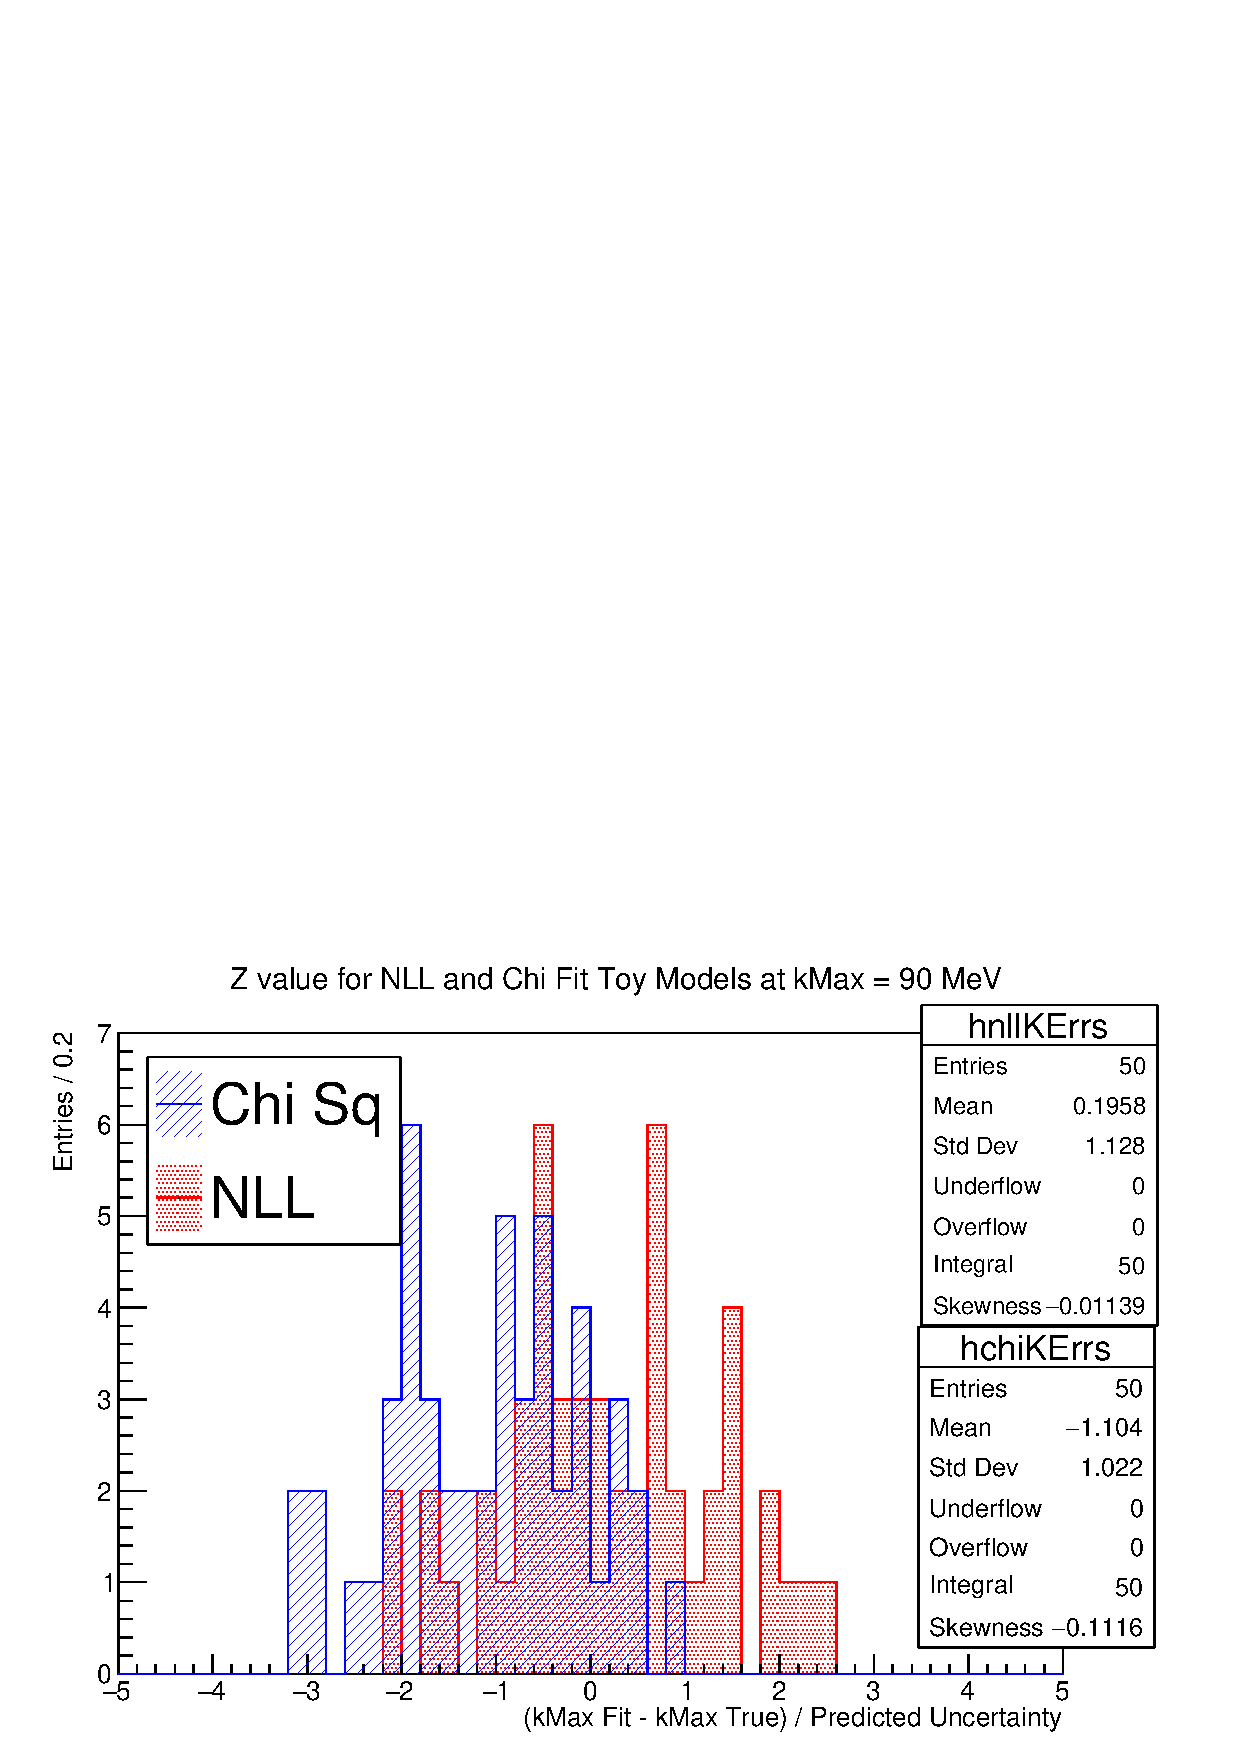
\includegraphics[width=0.48\linewidth]{figures/png/toy_kMax_z_values_1998_response.png}
%%   }
%%   \caption{Fit results z values for 50 toy data sets using the (a) 1992 or (b) 1998 detector response function.
%%     The toy data sets are generated from a convolution with an end point value of 90 MeV and generated
%%     with 1275 data points. The z value for a fit is the fit end point value minus the true value, divided
%%     by the fit estimated uncertainty. 
%%   }
%%   \label{fig:ToyFitZs}
%% \end{figure}



%%%%%%%%%%%%%%%%%%%%%%%%%%%%%%%%%%%%%%%%%%%%%%%%%%%%%%%%%%%%%%%%%%%%%%%%%%%%%%


\subsection { Fits of the 1992 data }
\begin{table}[h]
  \begin{center}
    \begin{tabular}{|l||l|l|l|l|l|l|}
      \hline
      Dataset & Published $k_{Max}$ & $\chi^2 / DoF$ & Our $k_{Max}$ & $\chi^2 / DoF$  & Response & Fit \\
      \hhline{|=||=|=|=|=|=|=|}
       Al 1992   & 90   $\pm$ 2   & 1.1 & 88.5 $\pm$ 0.5 &  1.6 (56.0 / 34) & 1992 & $\chi^2$ \\  
                 &                &     & 90.1 $\pm$ 0.5 &  1.2 (40.1 / 34) & 1998 & $\chi^2$ \\  
                                                                             
                 &                &     & 91.3 $\pm$ 0.4 & 2.3 ( 100.9 / 43)& 1992 & $\mathcal{L}$ \\
                 &                &     & 90.8 $\pm$ 0.5 & 1.5 ( 63.0 / 43) & 1998 & $\mathcal{L}$ \\
       \hline                                                                
       Ca 1992   & 93   $\pm$ 2   & 1.6 & 91.4 $\pm$ 0.4 &  2.6 (100.2 / 39)& 1992 & $\chi^2$ \\  
                 &                &     & 93.1 $\pm$ 0.4 &  1.4 (52.7 / 39) & 1998 & $\chi^2$ \\  
                                                                             
                 &                &     & 94.8 $\pm$ 0.3 & 4.6 ( 196.5 / 43)& 1992 & $\mathcal{L}$ \\
                 &                &     & 94.1 $\pm$ 0.4 & 1.7 ( 72.5 / 43) & 1998 & $\mathcal{L}$ \\
      \hline                                                                 
       Mo 1992   & 90   $\pm$ 2   & 0.8 & 88.3 $\pm$ 0.5 &  1.6 (50.3 / 32) & 1992 & $\chi^2$ \\  
                 &                &     & 89.3 $\pm$ 0.4 &  0.8 (24.7 / 32) & 1998 & $\chi^2$ \\  
                                                                             
                 &                &     & 90.1 $\pm$ 0.4 & 0.7 ( 29.2 / 43) & 1992 & $\mathcal{L}$ \\
                 &                &     & 90.5 $\pm$ 0.3 & 1.6 ( 70.9 / 43) & 1998 & $\mathcal{L}$ \\
      \hline                                                                 
       Pb 1992   & 84   $\pm$ 3   & 0.9 & 82.5 $\pm$ 0.5 &  1.3 (41.1 / 31) & 1992 & $\chi^2$ \\  
                 &                &     & 83.4 $\pm$ 0.5 &  0.6 (18.2 / 31) & 1998 & $\chi^2$ \\  
                                                                             
                 &                &     & 85.5 $\pm$ 0.4 & 2.1 ( 92.3 / 43) & 1992 & $\mathcal{L}$ \\
                 &                &     & 84.8 $\pm$ 0.5 & 0.7 ( 28.7 / 43) & 1998 & $\mathcal{L}$ \\
      \hline                                                                 
       Si 1992   & 92   $\pm$ 2   & 1.7 & 89.6 $\pm$ 0.4 &  3.1 (102.9 / 33)& 1992 & $\chi^2$ \\  
                 &                &     & 91.0 $\pm$ 0.4 &  1.3 (42.4 / 33) & 1998 & $\chi^2$ \\  
                                                                             
                 &                &     & 92.3 $\pm$ 0.3 & 3.4 ( 147.7 / 43)& 1992 & $\mathcal{L}$ \\
                 &                &     & 91.7 $\pm$ 0.4 & 1.2 ( 52.6 / 43) & 1998 & $\mathcal{L}$ \\
      \hline                                                                 
       Sn 1992   & 87   $\pm$ 2   & 1.1 & 85.6 $\pm$ 0.5 &  2.4 (74.7 / 31) & 1992 & $\chi^2$ \\  
                 &                &     & 86.9 $\pm$ 0.5 &  0.7 (21.7 / 31) & 1998 & $\chi^2$ \\  
                                                                             
                 &                &     & 88.4 $\pm$ 0.3 & 2.5 ( 109.6 / 43) & 1992 & $\mathcal{L}$ \\
                 &                &     & 87.7 $\pm$ 0.4 & 0.6 ( 26.6 / 43) & 1998 & $\mathcal{L}$ \\
      \hline                           
    \end{tabular}
  \end{center}
  \caption{The fit results.}
  \label{table:fits1992}
\end{table}

%%%%%%%%%%%%%%%%%%%%%%%%%%%%%%%%%%%%%%%%%%%%%%%%%%%%%%%%%%%%%%%%%%%%%%%%%%%%%%
\subsection { Fits of the 1995 data }

\begin{table}[h]
  \begin{center}
    \begin{tabular}{|l||l|l|l|l|l|l|}
      \hline
      Dataset & Published $k_{Max}$ & $\chi^2 / DoF$ & Our $k_{Max}$ & $\chi^2 / DoF$  & Response & Fit \\
      \hhline{|=||=|=|=|=|=|=|}
       Ag 1995   & 89.0 $\pm$ 3.2 & 1.2 &83.9 $\pm$ 0.7 &  2.0 (60.7 / 30)  & 1992 & $\chi^2$ \\  
                 &                &     &85.0 $\pm$ 0.7 &  1.0 (29.2 / 30)  & 1998 & $\chi^2$ \\  
                                                                             
                &                &     & 87.2 $\pm$ 0.4 & 2.2 ( 93.8 / 43) & 1992 & $\mathcal{L}$ \\
                &                &     & 86.3 $\pm$ 0.5 & 0.8 ( 35.9 / 43) & 1998 & $\mathcal{L}$ \\      
      \hline                                                                
       Al 1995   & 90.1 $\pm$ 1.8 & 1.5 &84.7 $\pm$ 0.3 &  4.2 (134.9 / 32) & 1992 & $\chi^2$ \\  
                 &                &     &85.3 $\pm$ 0.3 &  1.3 (41.9 / 32)  & 1998 & $\chi^2$ \\  
                                                                            
                &                &     & 87.2 $\pm$ 0.2 & 4.7 ( 203.1 / 43) & 1992 & $\mathcal{L}$ \\
                &                &     & 86.5 $\pm$ 0.3 & 1.3 ( 54.3 / 43) & 1998 & $\mathcal{L}$ \\
      \hline                                                                
       O 1995    & 88.4 $\pm$ 2.3 & 2.1 &83.3 $\pm$ 0.3 &  4.5 (113.5 / 25) & 1992 & $\chi^2$ \\  
                 &                &     &84.1 $\pm$ 0.3 &  1.3 (33.3 / 25)  & 1998 & $\chi^2$ \\  
                                                                            
                &                &     & 85.3 $\pm$ 0.2 & 3.6 ( 153.5 / 43)& 1992 & $\mathcal{L}$\\
                &                &     & 84.7 $\pm$ 0.3 & 1.1 ( 48.3 / 43) & 1998 & $\mathcal{L}$\\
      \hline                                                                     
       Si 1995   & 89.4 $\pm$ 1.8 & 2.7 &84.7 $\pm$ 0.3 &  4.9 (151.5 / 31) & 1992 & $\chi^2$ \\  
                 &                &     &85.2 $\pm$ 0.3 &  2.3 (71.9 / 31)  & 1998 & $\chi^2$ \\  
                                                                             
                &                &     & 87.3 $\pm$ 0.2 & 5.6 ( 241.5 / 43) & 1992 & $\mathcal{L}$ \\
                &                &     & 86.7 $\pm$ 0.3 & 2.4 ( 102.9 / 43)& 1998 & $\mathcal{L}$ \\
      \hline                                                                
       Ti 1995   & 89.2 $\pm$ 2.0 & 1.9 &84.8 $\pm$ 0.5 &  3.6 (116.0 / 32) & 1992 & $\chi^2$ \\  
                 &                &     &85.8 $\pm$ 0.4 &  1.5 (46.9 / 32)  & 1998 & $\chi^2$ \\  
                                                                            
                &                &     & 87.7 $\pm$ 0.3 & 3.9 ( 169.7 / 43) & 1992 & $\mathcal{L}$ \\
                &                &     & 86.9 $\pm$ 0.4 & 1.3 ( 57.4 / 43) & 1998 & $\mathcal{L}$ \\
      \hline                                                                
       Zr 1995   & 89.2 $\pm$ 3.4 & 1.2 &84.3 $\pm$ 0.6 &  2.9 (89.7 / 31)  & 1992 & $\chi^2$ \\  
                 &                &     &85.0 $\pm$ 0.6 &  1.6 (49.6 / 31)  & 1998 & $\chi^2$ \\  
                                                                            
                &                &     & 87.3 $\pm$ 0.4 & 2.9 ( 122.6 / 43) & 1992 & $\mathcal{L}$ \\
                &                &     & 86.4 $\pm$ 0.5 & 1.4 ( 59.4 / 43) & 1998 & $\mathcal{L}$ \\
      \hline
                                                                                
    \end{tabular}
  \end{center}
  \caption{The fit results.}
  \label{table:fits1995}
\end{table}


%%%%%%%%%%%%%%%%%%%%%%%%%%%%%%%%%%%%%%%%%%%%%%%%%%%%%%%%%%%%%%%%%%%%%%%%%%%%%%
\subsection { Fits of the 1998 data }
\begin{table}[h]
  \begin{center}
    \begin{tabular}{|l||l|l|l|l|l|l|}
      \hline
      Dataset & Published $k_{Max}$ & $\chi^2 / DoF$ & Our $k_{Max}$ & $\chi^2 / DoF$  & Response & Fit \\
      \hhline{|=||=|=|=|=|=|=|}
       Ni58 1998 & 92   $\pm$ 2   & 1.8 & 87.3 $\pm$ 0.6 &  2.3 (73.7 / 32) & 1992 & $\chi^2$ \\  
                 &                &     & 88.3 $\pm$ 0.6 &  1.0 (32.7 / 32) & 1998 & $\chi^2$ \\  
                                                                             
                &                 &     & 90.4 $\pm$ 0.4 & 2.5 ( 107.2 / 43) & 1992 & $\mathcal{L}$ \\
                &                 &     & 89.6 $\pm$ 0.5 & 0.9 ( 40.0 / 43) & 1998 & $\mathcal{L}$ \\
      \hline                                                                 
       Ni60 1998 & 92   $\pm$ 2   & 2.0 & 85.5 $\pm$ 0.5 &  2.6 (84.4 / 33) & 1992 & $\chi^2$ \\  
                 &                &     & 86.8 $\pm$ 0.5 &  1.1 (36.4 / 33) & 1998 & $\chi^2$ \\  
                                                                             
                &                 &     & 88.7 $\pm$ 0.3 & 3.5 ( 151.1 / 43) & 1992 & $\mathcal{L}$ \\
                &                 &     & 87.9 $\pm$ 0.4 & 1.1 ( 47.5 / 43) & 1998 & $\mathcal{L}$ \\
      \hline                                                                 
       Ni62 1998 & 90   $\pm$ 2   & 1.3 & 84.6 $\pm$ 0.6 &  1.7 (51.1 / 30) & 1992 & $\chi^2$ \\  
                 &                &     & 85.9 $\pm$ 0.6 &  0.8 (25.1 / 30) & 1998 & $\chi^2$ \\  
                                                                             
                &                 &     & 87.7 $\pm$ 0.4 & 2.1 ( 89.2 / 43) & 1992 & $\mathcal{L}$ \\
                &                 &     & 87.0 $\pm$ 0.5 & 0.7 ( 30.9 / 43) & 1998 & $\mathcal{L}$ \\
      \hline                           
    \end{tabular}
  \end{center}
  \caption{The fit results.}
  \label{table:fits1998}
\end{table}

%%%%%%%%%%%%%%%%%%%%%%%%%%%%%%%%%%%%%%%%%%%%%%%%%%%%%%%%%%%%%%%%%%%%%%%%%%%%%%
\subsection { Fits of the 1999 data }

\begin{table}[h]
  \begin{center}
    \begin{tabular}{|l||l|l|l|l|l|l|}
      \hline
      Dataset & Published $k_{Max}$ & $\chi^2 / DoF$ & Our $k_{Max}$ & $\chi^2 / DoF$  & Response & Fit \\
      \hhline{|=||=|=|=|=|=|=|}
       O 1999    & 88.4 $\pm$ 2.3 & 2.1 & 84.8 $\pm$ 0.4 &  5.6 (157.1 / 28)& 1992 & $\chi^2$ \\  
                 &                &     & 86.0 $\pm$ 0.4 &  1.7 (46.7 / 28) & 1998 & $\chi^2$ \\  
                                                                             
                 &                &     & 87.2 $\pm$ 0.2 & 5.0 ( 213.4 / 43)& 1992 & $\mathcal{L}$\\
                 &                &     & 86.6 $\pm$ 0.3 & 2.2 ( 93.9 / 43) & 1998 & $\mathcal{L}$\\
      \hline                                                                 
       Ti 1999   & 89.2 $\pm$ 2.0 & 1.9 & 86.3 $\pm$ 0.5 &  3.7 (123.0 / 33)& 1992 & $\chi^2$ \\  
                 &                &     & 87.5 $\pm$ 0.4 &  1.4 (47.7 / 33) & 1998 & $\chi^2$ \\  
                                                                             
                 &                &     & 89.3 $\pm$ 0.3 & 4.2 ( 179.0 / 43) & 1992 & $\mathcal{L}$ \\
                 &                &     & 88.5 $\pm$ 0.4 & 1.2 ( 52.1 / 43) & 1998 & $\mathcal{L}$ \\
      \hline                           
    \end{tabular}
  \end{center}
  \caption{The fit results.}
  \label{table:fits1999}
\end{table}



